\documentclass[11pt]{standalone}

\usepackage[T1]{fontenc}
\usepackage[utf8]{inputenc}

\usepackage{amsfonts}
\usepackage{amsmath, amssymb}
\usepackage{mathtools}
\usepackage{textcomp} % Needed for symbols such as degrees, copyright, etc.
\usepackage[gen]{eurosym}
\usepackage{ar}

% \usepackage[scale=1.09,textlf,mathlf,swash]{MinionPro}
% \usepackage[scale=1.09]{MyriadPro}

\usepackage{tikz,pgfplots}
\usetikzlibrary{arrows,shapes,positioning,shadows,trees,patterns,intersections,matrix,fit,backgrounds}
\pgfplotsset{compat=newest}
  \pgfplotsset{plot coordinates/math parser=false}
\newlength\figureheight
    \newlength\figurewidth
\usepackage{tikz-3dplot}
\usepackage{tkz-euclide}
\tikzset{
  basic box/.style={
    shape=rectangle, rounded corners, align=center,
    draw=#1, fill=#1!25},
}

% \usepackage[table,pdftex]{xcolor}

\definecolor{MITred}{RGB}{163, 31, 52} % #a31f34
\definecolor{MITdg}{RGB}{138, 139, 140}
\definecolor{MITlg}{RGB}{194, 192, 191}
\definecolor{AAblue}{RGB}{0, 23, 63}
\definecolor{AAgray}{RGB}{123, 118, 117}
\definecolor{AAlb}{RGB}{0, 135, 188}
\definecolor{AAMITmix}{RGB}{82, 27, 58}

\definecolor{red}{HTML}{AD1737}
\definecolor{brown}{HTML}{990000}
\definecolor{bar}{HTML}{8D9965}

\definecolor{AAblue2}{RGB}{0, 71, 117} % #004775

\colorlet{AAMITmix2}{AAblue2!50!MITred}

\definecolor{redc}{RGB}{230, 50, 50}
\definecolor{bluec}{RGB}{0, 70, 150}
\definecolor{greenc}{RGB}{50, 140, 80}

% color schemes
%   continuous (4)
\colorlet{cont41}{MITred}
\colorlet{cont42}{MITred!65}
\colorlet{cont43}{AAblue2!65}
\colorlet{cont44}{AAblue2}

%   continuous (5)
\colorlet{cont51}{MITred}
\colorlet{cont52}{MITred!75!white}
\colorlet{cont53}{AAMITmix2!75!white}
\colorlet{cont54}{AAblue2!75!white}
\colorlet{cont55}{AAblue2}

%   continuous (6)
\colorlet{cont61}{MITred}
\colorlet{cont62}{MITred!85!white}
\colorlet{cont63}{MITred!60!white}
\colorlet{cont64}{AAblue2!60!white}
\colorlet{cont65}{AAblue2!85!white}
\colorlet{cont66}{AAblue2}

%   continuous (7)
\colorlet{cont71}{MITred}
\colorlet{cont72}{MITred!85!white}
\colorlet{cont73}{MITred!65!white}
\colorlet{cont74}{AAMITmix2!50!white}
\colorlet{cont75}{AAblue2!65!white}
\colorlet{cont76}{AAblue2!85!white}
\colorlet{cont77}{AAblue2}

%   continuous (8)
\colorlet{cont81}{MITred}
\colorlet{cont82}{MITred!85!white}
\colorlet{cont83}{MITred!70!white}
\colorlet{cont84}{MITred!55!white}
\colorlet{cont85}{AAblue2!55!white}
\colorlet{cont86}{AAblue2!70!white}
\colorlet{cont87}{AAblue2!85!white}
\colorlet{cont88}{AAblue2}

%   continuous (9)
\colorlet{cont91}{MITred}
\colorlet{cont92}{MITred!87!white}
\colorlet{cont93}{MITred!75!white}
\colorlet{cont94}{MITred!63!white}
\colorlet{cont95}{AAMITmix2!50!white}
\colorlet{cont96}{AAblue2!63!white}
\colorlet{cont97}{AAblue2!75!white}
\colorlet{cont98}{AAblue2!87!white}
\colorlet{cont99}{AAblue2}

%   qualitative (4)
\colorlet{qual41}{MITred}
\colorlet{qual44}{AAblue2}
\definecolor{qual42}{RGB}{0,163,136}
\definecolor{qual43}{RGB}{163,84,31}

%   qualitative (5)
% \colorlet{qual51}{MITred}
% \colorlet{qual55}{AAblue2}
% \definecolor{qual52}{RGB}{234, 110, 68}
% \definecolor{qual53}{RGB}{235, 210, 113}
% \definecolor{qual54}{RGB}{35, 133, 135}
\colorlet{qual55}{AAblue2}
\definecolor{qual54}{RGB}{166,206,227}
\definecolor{qual53}{RGB}{251,154,153}
\colorlet{qual51}{MITred}
\colorlet{qual52}{qual53!50!qual51}

\definecolor{qual61}{RGB}{166,206,227}
\colorlet{qual62}{AAblue2}
\definecolor{qual63}{RGB}{178,223,138}
\definecolor{qual64}{RGB}{51,160,44}
\definecolor{qual65}{RGB}{251,154,153}
\colorlet{qual66}{MITred}

\newcommand{\overbar}[1]{\mkern 1.5mu\overline{\mkern-1.5mu#1\mkern-0.75mu}\mkern 0.75mu}

\DeclareMathOperator*{\argmin}{arg\,min}


\tikzstyle{powder}=[black!20]

\begin{document}

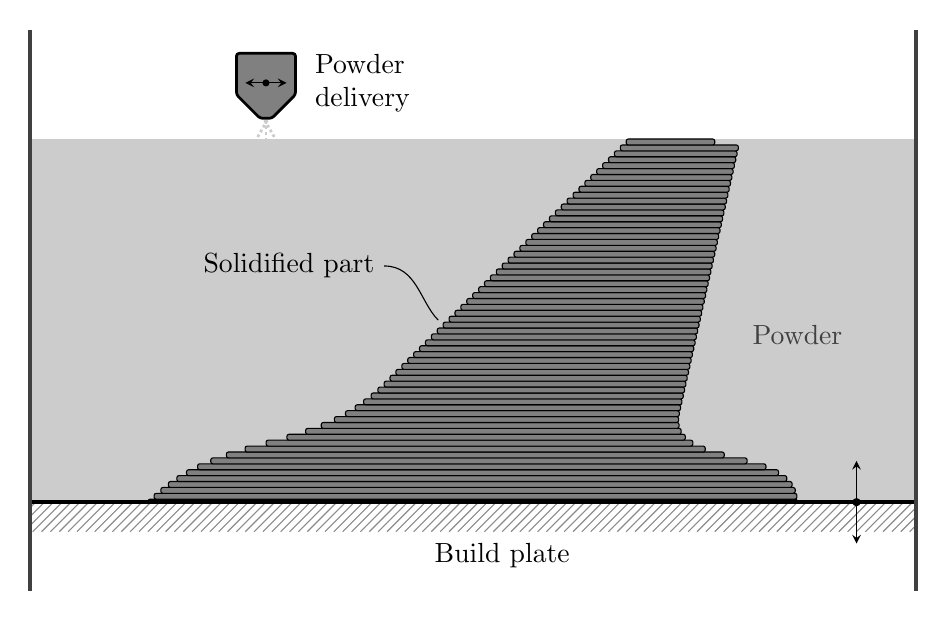
\begin{tikzpicture}[scale=1.5,>=stealth]

  \draw[draw=none,name path=LE] (-3,0) to[out=45,in=-135] (-1,1) -- (1,3); % leading edge
  \draw[draw=none,] (1,3) -- (2,3); % top
  \draw[draw=none,name path=TE] (2,3) -- (1.5,0.75) to[out=-101.3099,in=90] (2.5,0); % trailing edge

  % powder
  \fill[powder] (-4,0) rectangle (3.5,3.075);

  \foreach \y in {0,0.05,...,3.01} {
    \draw[draw=none,name path=temp] (-4,\y) -- (3.5,\y);
    \path [name intersections={of=LE and temp,by=A}];
    \path [name intersections={of=TE and temp,by=B}];
    \draw (A) -- (B);
    \draw[rounded corners=0.75pt,fill=black!50] ($(A)+(0,-0.025)$) rectangle ($(B)+(0,0.025)$);
  }

  % draw top layer
  \draw[rounded corners=0.75pt,fill=black!50] (1.05,3.025) -- (1.8,3.025) -- (1.8,3.075) -- (1.05,3.075) -- cycle;

  % base
  \fill [white] (-4,-0.25) rectangle (3.5,0);
  \begin{scope}
    \clip (-4,-0.25) rectangle (3.5,0);
    \foreach \x in {-6,-5.925,...,4} { \draw[MITdg] (\x,-0.25) -- ++(45:1); }
  \end{scope}
  \draw [black,line width=1.5pt] (-4,0) -- (3.5,0);

  % draw sides
  \draw [black!75,line width=1.5pt] (-4,4) -- (-4,-0.75);
  \draw [black!75,line width=1.5pt] (3.5,-0.75) -- (3.5,4);

  \draw[<->] (3,-0.35) -- (3,0.35);
  \fill (3,0) circle (1pt);

  % powder depositer
  \begin{scope}[shift={(-2,3.25)}]
    % powder
    \draw[powder,line width=1pt,dash pattern=on 1pt off 1pt] (-0.035,0.025) -- ++ (-60:0.3);
    \draw[powder,line width=1pt,dash pattern=on 1pt off 1pt] (0,0.025) -- ++ (-90:0.3);
    \draw[powder,line width=1pt,dash pattern=on 1pt off 1pt] (0.035,0.025) -- ++ (-120:0.3);

    \draw[line width=1pt,rounded corners=1pt,fill=black!50] (-0.05,0) -- (0.05,0) -- (0.25,0.2) -- (0.25,0.55) -- (-0.25,0.55) -- (-0.25,0.2) -- cycle;

    % movement
    \draw[fill=black] (0,0.3) circle (0.025);
    \draw[<->] (-0.175,0.3) -- (0.175,0.3);
    % \draw[<->] (0,0.125) -- (0,0.475);
  \end{scope}

  % Build plate annotation
  \node at (0,-0.45) {Build plate};

  % Powder annotation
  \node[above,black!75] at (2.5,1.25) {Powder};

  % Powder delivery
  \node[right,anchor=west,shift={(0.5,0.45)},align=left] at (-2,3.25) {Powder\\ delivery};

  % Part annotation
  \draw[shorten <=2.5pt] (-0.5,1.5) to[out=135,in=0] node[at end,left,align=right] {Solidified part}(-1,2);

\end{tikzpicture}

\end{document}
